\documentclass[12pt]{article}\usepackage[]{graphicx}\usepackage[]{color}
%% maxwidth is the original width if it is less than linewidth
%% otherwise use linewidth (to make sure the graphics do not exceed the margin)
\makeatletter
\def\maxwidth{ %
  \ifdim\Gin@nat@width>\linewidth
    \linewidth
  \else
    \Gin@nat@width
  \fi
}
\makeatother

\definecolor{fgcolor}{rgb}{0.345, 0.345, 0.345}
\newcommand{\hlnum}[1]{\textcolor[rgb]{0.686,0.059,0.569}{#1}}%
\newcommand{\hlstr}[1]{\textcolor[rgb]{0.192,0.494,0.8}{#1}}%
\newcommand{\hlcom}[1]{\textcolor[rgb]{0.678,0.584,0.686}{\textit{#1}}}%
\newcommand{\hlopt}[1]{\textcolor[rgb]{0,0,0}{#1}}%
\newcommand{\hlstd}[1]{\textcolor[rgb]{0.345,0.345,0.345}{#1}}%
\newcommand{\hlkwa}[1]{\textcolor[rgb]{0.161,0.373,0.58}{\textbf{#1}}}%
\newcommand{\hlkwb}[1]{\textcolor[rgb]{0.69,0.353,0.396}{#1}}%
\newcommand{\hlkwc}[1]{\textcolor[rgb]{0.333,0.667,0.333}{#1}}%
\newcommand{\hlkwd}[1]{\textcolor[rgb]{0.737,0.353,0.396}{\textbf{#1}}}%

\usepackage{framed}
\makeatletter
\newenvironment{kframe}{%
 \def\at@end@of@kframe{}%
 \ifinner\ifhmode%
  \def\at@end@of@kframe{\end{minipage}}%
  \begin{minipage}{\columnwidth}%
 \fi\fi%
 \def\FrameCommand##1{\hskip\@totalleftmargin \hskip-\fboxsep
 \colorbox{shadecolor}{##1}\hskip-\fboxsep
     % There is no \\@totalrightmargin, so:
     \hskip-\linewidth \hskip-\@totalleftmargin \hskip\columnwidth}%
 \MakeFramed {\advance\hsize-\width
   \@totalleftmargin\z@ \linewidth\hsize
   \@setminipage}}%
 {\par\unskip\endMakeFramed%
 \at@end@of@kframe}
\makeatother

\definecolor{shadecolor}{rgb}{.97, .97, .97}
\definecolor{messagecolor}{rgb}{0, 0, 0}
\definecolor{warningcolor}{rgb}{1, 0, 1}
\definecolor{errorcolor}{rgb}{1, 0, 0}
\newenvironment{knitrout}{}{} % an empty environment to be redefined in TeX

\usepackage{alltt}
\usepackage{natbib}
\usepackage{color}
\usepackage[dvipsnames,svgnames*]{xcolor}
\usepackage{array}
\usepackage[colorlinks=TRUE, linkcolor=blue]{hyperref}
\usepackage[font=small,skip=5pt]{caption}
\usepackage[aboveskip=2pt]{subcaption}
\usepackage{graphicx}
\usepackage{amsmath}
\usepackage{amsthm}
\usepackage{amsfonts}
\usepackage{url}
\usepackage{ulem}
\usepackage{afterpage}
\usepackage{bbm}

\graphicspath{{images/}}
\DeclareGraphicsRule{.tif}{png}{.png}{`convert #1 `dirname #1`/`basename #1 .tif`.png}
\IfFileExists{upquote.sty}{\usepackage{upquote}}{}
\begin{document}


\section{Variational Bayes - Normal Mixture Model}

We have $iid$ observations $y_i$ genrated by a two level Normal Mixture Model with means $\mu_1 \mbox{ and } \mu_2$ and known variance $1$, so

$$p(y_i | \mu_1, \mu_2, k_i) = \mathcal{N}(\mu_1, 1)^{k_i} \mathcal{N}(\mu_2, 1)^{1-k_i}.$$

where the latent variable $k_i = 1$ if $y_i$ is drawn from $\mathcal{N}(\mu_1, 1)$ and $k_i = 0$ otherwise.

Further, $\bold{k}$ is modelled as $iid$ Bernoulli with parameter $\pi$, so
$$p(k_i | \pi) = \pi^{k_i} (1-\pi)^{1-k_i}. $$

Introducing the priors $p(\pi) \sim U(0, 1)$ and $p(\mu_1, \mu_2) \propto 1$, the joint distribution becomes
\begin{eqnarray}
\label{1}
p(y, k, \mu_1, \mu_2, \pi) & = & \prod^{n}_{i=1} p(y_i | k_i, \mu_1, \mu_2, \pi) p(k_i | \pi) p(\pi) p(\mu_1 \mu_2) \nonumber \\
& \propto & \prod^{n}_{i=1} \left(\frac{1}{\sqrt{2\pi}} \exp \left\{\frac{-(y_i-\mu_1)^2}{2}\right\}\right)^{k_i} \left(\frac{1}{\sqrt{2\pi}} \exp \left\{\frac{-(y_i-\mu_2)^2}{2}\right\}\right)^{1-k_i} \nonumber \\
& \times & \pi^{k_i} (1-\pi)^{1-k_i} \nonumber \\
\ln(p(y, k, \mu_1, \mu_2, \pi)) & = & \sum_{i=1}^{N} \left[ \ln\left(\exp \left\{\frac{-(y_i-\mu_1)^2}{2}\right\}^{k_i}\right)\right] + \sum_{i=1}^{N} \left[ \ln\left(\exp \left\{\frac{-(y_i-\mu_2)^2}{2}\right\}^{1-k_i}\right)\right] \nonumber \\
& + & \sum_{i=1}^{N} k_i \ln(\pi) + \sum_{i=1}^{N} (1-k_i) \ln(1-\pi) \nonumber \\
& = & \sum_{i=1}^{N} \left[ k_{i} \frac{-(y_i-\mu_1)^2}{2}\right] + \sum_{i=1}^{N} \left[ (1-k_{i}) \frac{-(y_i-\mu_2)^2}{2}\right] \nonumber \\
& + & \sum_{i=1}^{N} k_i \ln(\pi) + \sum_{i=1}^{N} (1-k_i) \ln(1-\pi) + c.
\end{eqnarray}

We can take the variational approximation factorisation $q(k_{1:n}, \mu_1, \mu_2, \pi) = \prod_{i=1}^{n} q(k_i)q(\mu_1)q(\mu_2)q(\pi)$, which implies independence of $k_i, k_j$ for $i \neq j$:

It can be shown that the factorisable distribution that minmises the KL Divergence between $q(\theta)$ and $p(\theta|y)$ satisfies

\begin{equation}
\label{2}
q_{i} \propto \exp (\mathbb{E}_{q_{j \neq i}} (\ln(p(y, x, \theta))))
\end{equation}

for all $q_{i}$, where $y$ is the observed data, $x$ is a latent variable and $\theta$ is a vector of unknown parameters.

Substituting (\ref{1}) into (\ref{2}) yields

\begin{eqnarray*}
\ln(q(\pi)) & = & \mathbb{E}_{k_{1:n}} \left[ \sum_{i=1}^{n} k_i \ln(\pi) + (1-k_i) \ln(1-\pi) + c \right] \\
& = & \sum_{i=1}^{n} \mathbb{E}(k_i) \ln (\pi) + (n- \sum_{i=1}^{n}\mathbb{E}(k_i)) \ln(1-\pi) + c \\
& = & \ln(\pi^{\sum_{i=1}^{n}\mathbb{E}(k_i)}(1-\pi)^{n-\sum_{i=1}^{n}\mathbb{E}(k_i)}) + c\\
q(\pi) & \propto & \pi^{\sum_{i=1}^{n}\mathbb{E}(k_i)}(1-\pi)^{n-\sum_{i=1}^{n}\mathbb{E}(k_i)} 
\end{eqnarray*}

Recognizing the kernel of a Beta distribution, we see that $q(\pi) \sim  \mathcal{B} (\alpha = \sum_{i=1}^{n} \mathbb{E}(k_i)+1, \beta = n-\sum_{i=1}^{n}\mathbb{E}(k_i) + 1)$. Continuing, we can find

\begin{eqnarray*}
\ln(q(\mu_1)) & = & \mathbb{E}_{k_{1:n}} \sum_{i=1}^{n} -k_i \frac{(y_i-\mu_1)^2}{2} + c  \\
& = & -\frac{1}{2} \left(\sum_{i=1}^{n}\mathbb{E}(k_i) (y_i-\mu_{1})^2\right) + c \\ 
& = & -\frac{1}{2}\left(\sum_{i=1}^{n}\mathbb{E}(k_i) ((y_i - \tilde{y}_1) + (\tilde{y}_1 - \mu_1))^2 \right)+ c \\
& = & -\frac{1}{2}\left(\sum_{i=1}^{n}\mathbb{E}(k_i) ((y_i - \tilde{y}_1)^2 + (\tilde{y}_1 - \mu_1)^2 - 2(y_i - \tilde{y}_1)(\tilde{y}_1 - \mu_1))\right) + c.
\end{eqnarray*}

Where
$$\tilde{y}_1 = \frac{\sum_{i=1}^{n} \mathbb{E}(k_i)y_i}{\sum_{i=1}^{n} \mathbb{E}(k_i)}.$$

Note that
$$\sum_{i=1}^{n}\mathbb{E}(k_i)(y_i - \tilde{y}_1) = \sum_{i=1}^{n}\mathbb{E}(k_i)\left(y_i - \frac{\sum_{i=1}^{n} \mathbb{E}(k_i)y_i}{\sum_{i=1}^{n} \mathbb{E}(k_i)}\right) = 0,$$

hence 
\begin{eqnarray*}
\ln(q(\mu_1)) & = & -\frac{\sum_{i=1}^{n}\mathbb{E}(k_i) (\tilde{y}_1-\mu_{1})^2}{2} + c.
\end{eqnarray*}


Recognizing the kernel of a Gaussian distribution, we can see that $q(\mu_1) \sim \mathcal{N} (\bar{\mu}_{1} = \tilde{y}_1, \lambda_{1} = (\sum_{i=1}^{n}\mathbb{E}(k_i)^{-1}).$
Similarly, $q(\mu_2) \sim \mathcal{N} (\bar{\mu}_{2} = \tilde{y}_2, \lambda_{2} = \sum_{i=1}^{n}\mathbb{E}(1-k_i)^{-1}))$ with
$$\tilde{y_2} = \frac{\sum_{i=1}^{n} \mathbb{E}(1-k_i)y_i}{\sum_{i=1}^{n} \mathbb{E}(1-k_i)}.$$

Through independence, all $q(k_i)$ have the same form,

\begin{eqnarray*}
\ln(q(k_i)) & = & \mathbb{E}_{\mu_1, \mu_2, \pi} \left[ k_{i} \frac{-(y_i-\mu_1)^2}{2} + (1-k_{i}) \frac{-(y_i-\mu_2)^2}{2} + k_i \ln(\pi) + (1-k_i) \ln(1-\pi) + c \right]\\
& = & k_i\frac{\mathbb{E}_{\mu_1} -(y_i-\mu_1)^2}{2}  + (1-k_i) \frac{\mathbb{E}_{\mu_2} -(y_i-\mu_2)^2}{2}  + k_i \mathbb{E}_\pi \ln(\pi) + (1-k_i) \mathbb{E}_\pi \ln(1-\pi) + c \\
& = & k_i \frac{2\tilde{\pi}_1-((y_i - \bar{\mu}_1)^2 + \lambda_1)}{2} + (1-k_i) \frac{2\tilde{\pi}_2-((y_i - \bar{\mu}_2)^2 + \lambda_2)}{2} + c\\
q(k_i) & \propto & \exp \left\{\frac{2\tilde{\pi}_1-((y_i - \bar{\mu}_1)^2 + \lambda_1)}{2} \right\}^{k_i} \exp \left\{\frac{2\tilde{\pi}_2-((y_i - \bar{\mu}_2)^2 + \lambda_2)}{2} \right\}^{1-k_i}
\end{eqnarray*}

The quantity $\tilde{\pi}_1 = \mathbb{E}_\pi \ln(\pi) = \psi(\alpha)-\psi(\alpha+\beta)$, and $\tilde{\pi}_2 = \mathbb{E}_\pi \ln(1-\pi) = \psi(\beta)-\psi(\alpha+\beta)$, where $\psi(\cdot)$ is the digamma function (Archambeau and Verleysen 2007). We also expanded the quadratic term and substitued in $(y_i^2 - \bar{\mu}_j)^2 + \lambda_j$ for $\mathbb{E} (y_i-\mu_j)^2$.


Each $k_i$ has a Bernoulli distribution with parameters $p_i = \exp \left\{\frac{2\tilde{\pi}_1-((y_i - \bar{\mu}_1)^2 + \lambda_1)}{2} \right\}, \mbox{ and } q_i = \exp \left\{\frac{2\tilde{\pi}_2-((y_i - \bar{\mu}_2)^2 + \lambda_2)}{2} \right\}.$

This gives us the update rules for the Variational Bayes iterations:

\begin{eqnarray*}
a & = & \sum_{i=1}^{n} \frac{p_i}{p_i+q_i} + 1 \\
b & = & \sum_{i=1}^{n} \frac{q_i}{p_i+q_i} + 1 \\
\bar{\mu}_1 & = &  \frac{\sum_{i=1}^{n} y_i p_i /(p_i+q_i)}{\sum_{i=1}^{n} p_i /(p_i+q_i)} \\
\lambda_1 & = & \left(\sum_{i=1}^{n} \frac{p_i}{p_i+q_i}\right)^{-1} \\
\bar{\mu}_2 & = &  \frac{\sum_{i=1}^{n} y_i q_i /(p_i+q_i)}{\sum_{i=1}^{n} q_i /(p_i+q_i)} \\
\lambda_2 & = & \left(\sum_{i=1}^{n} \frac{q_i}{p_i+q_i}\right)^{-1} \\
p_i & = & \exp \left\{\frac{2(\psi(a)-\psi(a+b))-((y_i - \bar{\mu}_1)^2 + \lambda_1)}{2} \right\} \\
q_i & = & \exp \left\{\frac{2(\psi(b)-\psi(a+b))-((y_i - \bar{\mu}_2)^2 + \lambda_2)}{2} \right\}
\end{eqnarray*}

\begin{knitrout}
\definecolor{shadecolor}{rgb}{0.969, 0.969, 0.969}\color{fgcolor}
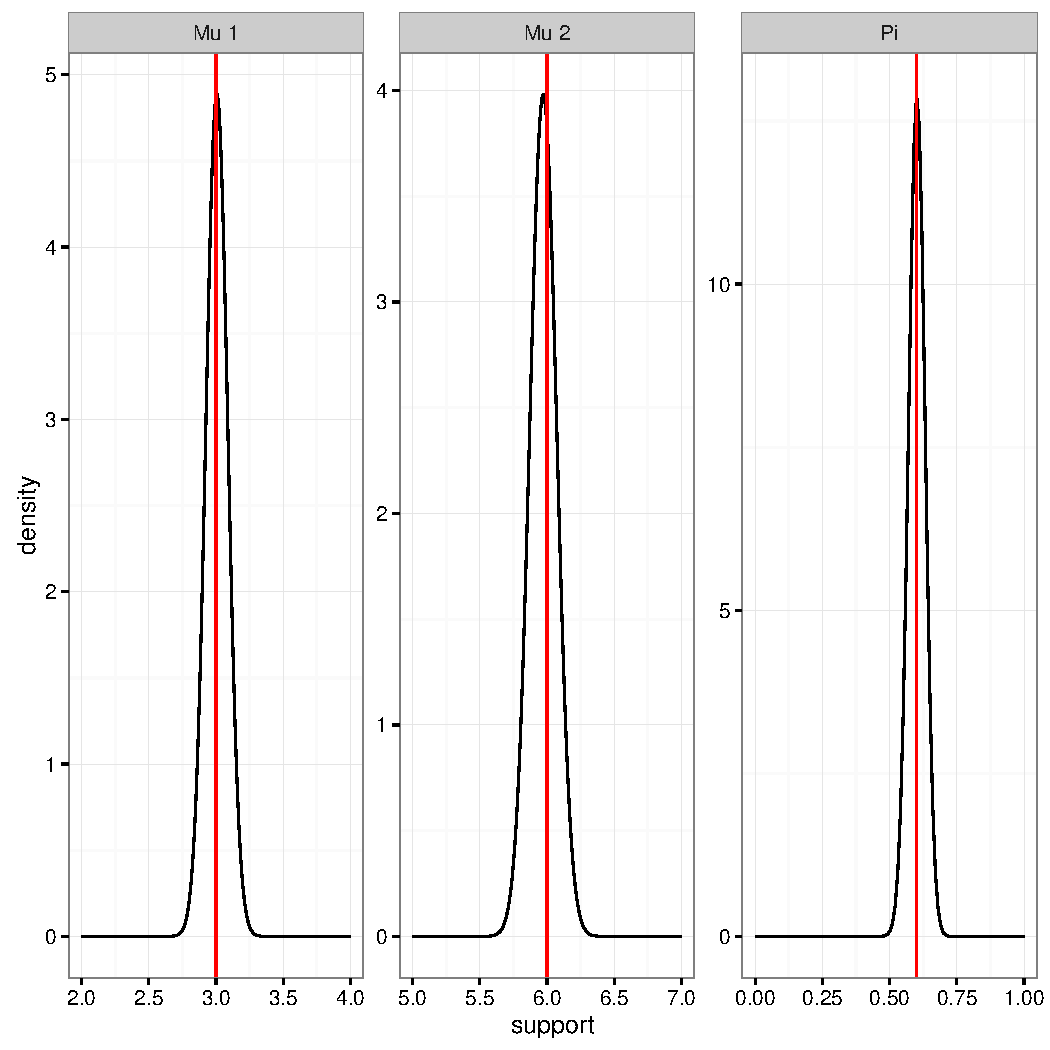
\includegraphics[width=\maxwidth]{figure/vbayes-1} 

\end{knitrout}
250 draws were simulated with parameters $\mu_1 = 3, \mu_2 = 6, \pi=0.6$ and th e variational algorithm was ran. After manually correcting mislabeling, $y_i$ was allocated to distribution 1 if $p_i > q_i$ and to distribution 2 if $p_i < q_i$, resulting in the successful classification of 235/250 draws. A more trivial decision rule to allocate $y_i$ to distribution 1 if $y_i < \bar{y}$ and to distribution 2 if $y_i > \bar{y}$ successfully classified 234/250 draws.

\begin{knitrout}
\definecolor{shadecolor}{rgb}{0.969, 0.969, 0.969}\color{fgcolor}
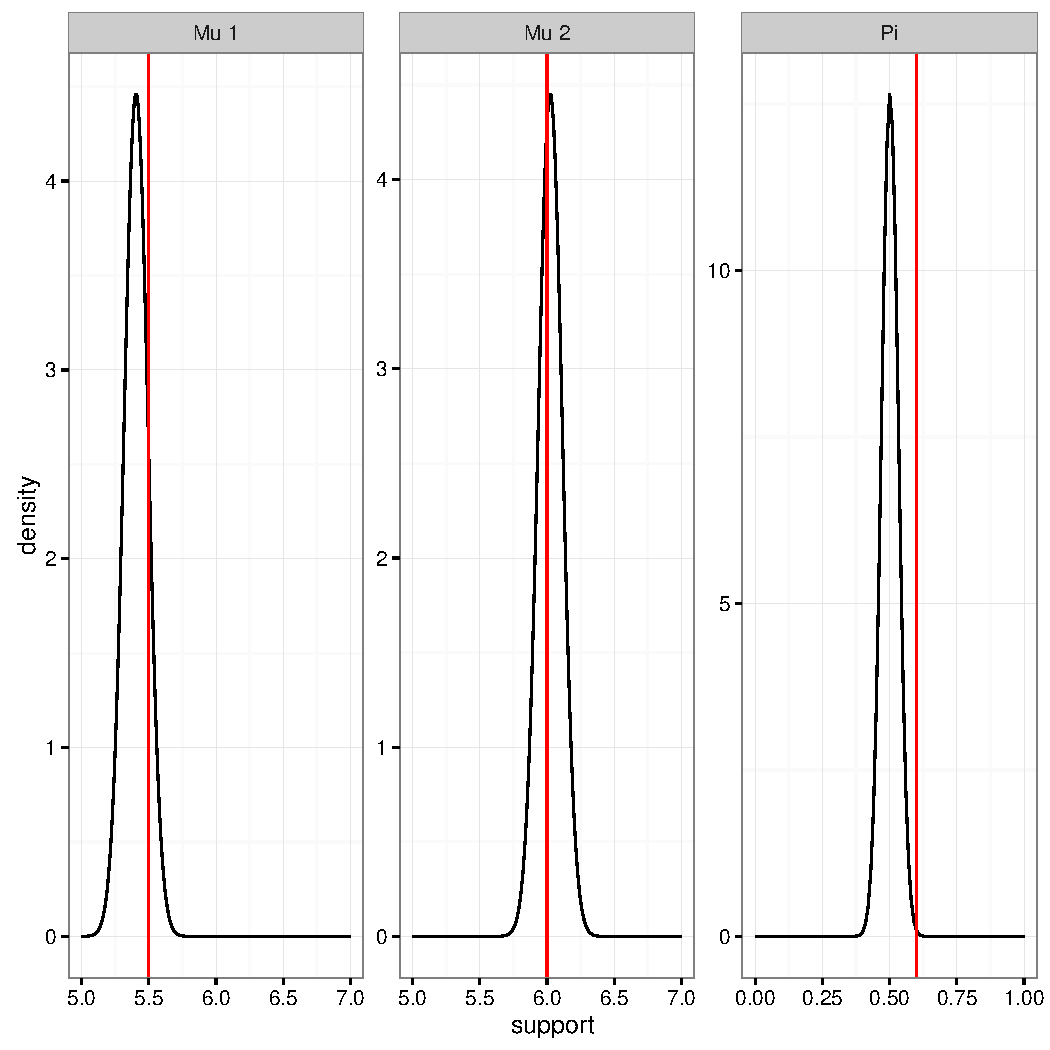
\includegraphics[width=\maxwidth]{figure/vbayes2-1} 

\end{knitrout}
250 draws were simulated with parameters $\mu_1 = 5.5, \mu_2 = 6, \pi=0.6$ to try and force an overlap in the data. $y_i$ was allocated to distribution 1 if $p_i > q_i$ and to distribution 2 if $p_i < q_i$, resulting in the successful classification of 158/250 draws. The trivial decision rule had identical classifications.

\end{document}
